\chapter{Introduction}

%TODO: What is Multi-Agent Reinforcement Learning (MARL)

\chapter{Motivation}

Most reviewed papers concerning MARL algorithms do not provide detailed experiments with huge groups of agents. This raises the question how agent policies behave in terms of metrics and visible wrong behavior when watching these agents play. Since the joint action as well as the communicated state increase with the number of agents, it is interesting how already developed algorithms perform. PyMARL is a collection of algorithms running on the SMAC environment which allows for multi-agent micro-management learning in StarCraftII. This is a novelty since most algorithms perform on different environments and are therefore not suitable for comparison. PyMARl combines already five algorithms (IQL,VDN,QMIX,COMA,QTRAN) while others have forked PyMARL or SMAC to run experiments (CKL, SMIX). Use of local and global rewards is not always consistent (f.e. some papers seem to use local rewards with algorithm A while others f.e. PyMARL implement algorithm A with global reward)


\chapter{Presets}

\section{PyMARL - A multi-agent reinforcement learning framework}

In order to setup PyMARL(fork) with extensions on local and combined rewards, the Readme in the following repository \url{https://github.com/PMatthaei/pymarl} contains a step by step guide. The main repository of PyMARL can be found at \url{https://github.com/oxwhirl/pymarl}. \cite{samvelyan19smac}

\section{Related work}

%TODO:What are algorithms doing? What are problems?

\subsection{Q-Learning in single agent environments}
%TODO: What is Q-Learning trying to achieve? What are problems? $\rightarrow$ MARL affected?

Q-Learning is an algorithm to find a suitable policy to maximize an agent`s accumulated long term reward without explicit information about dynamics of the environment including the reward scheme. Q-learning estimates the value of an action in a particular state of the environment.\cite{watkins1989learning}

\makebox[\textwidth]{
	$Q_{\text {new}}\left(s_{t}, a_{t}\right) 
	\leftarrow 
	\underbrace{Q\left(s_{t}, a_{t}\right)}_{\text {old value}}
	+
	\underbrace{\alpha}_{\text {learning rate}}
	\cdot
	\overbrace{
		(\underbrace{
			\underbrace{r_{t}}_{\text {reward}}
			+
			\underbrace{\gamma}_{\text {discount factor}}
			\cdot
			\underbrace{\max _{a} Q\left(s_{t+1}, a\right)}_{\text{estimate of optimal future value}}
		}_{\text {new value (temporal difference target)}} -
		\underbrace{Q\left(s_{t}, a_{t}\right)}_{\text {old value}})
	}^{\text{temporal difference}}$
}


\subsection{DQN - Deep Q-Networks}
%TODO: Summarize DQNs
\cite{lin1993reinforcement}

\subsection{IQL - Independent Q-Learning}

% Description of paper, basic ideas, main formulas
Each agent deploys an independent Q-learning algorithm to learn an individual action-value function solely based on their own actions.

Recently DQN have been used to estimate the value-function especially in environments with large input \cite{tampuu2017multiagent}. In a multi-agent setup, the taken action is determined by the corresponding DQN for all agents separately, therefore the environment is the only interface for interaction between agents. This results in an easy to setup architecture which is decentralized, stable across tasks and computational efficient. The setup by \cite{tampuu2017multiagent} uses local rewards and the game state (screen capture of the game itself) is fully observable shared between the agents.
This results in the update rule for a single agent \textit{i}:

% Formulas
\begin{center}

$Q^{\text {i}}_{new}\left(s^{i}_{t}, a^{i}_{t}\right) 
\leftarrow 
Q^{i}\left(s^{i}_{t}, a^{i}_{t}\right)
+
\alpha
\cdot
(r^{i}_{t}+\gamma\cdot\max _{a} Q\left(s_{t+1}, a\right)
-
Q^{i}\left(s^{i}_{t}, a^{i}_{t}\right)
$
	
\end{center}

% Discussion
Although this implementation is straight forward and simple, simultaneous learning and exploring agents create a non-stationarity in the environment. This can lead to non-convergence of policies and inaccurate representation of interactions between agents \cite{rashid2018qmix}.

% Implementation in PyMARL
%TODO: describe how similar, what is different?
The implementation of IQL in PyMARL is similar to the previous setup. The state for this setup is a (partial) copy of the game`s state as opposed to image data as in above setup.

%TODO: Summarize Tan 1993
%
% IQL Tan 1993
%
%- Comparsion of three methods: 
%
%	- sharing state,actions,rewards triplets, state space increases exponentially in term of number of agents
%	
%	- sharing episodes (sequence of triplets), not always possible for heterogeneous agents
%	
%	-sharing policies
%Assuming a independent task (deer hunt):
%- sensation from other agents is beneficial if used efficiently f.e.use hunter sensation first, if he cannot see prey, use scouts sensation, decreasing sensation range hindered training, short sighted scouts lose track before coop agent can follow, leading him to nowhere
%
%- sharing episodes and policies speeds up learning at cost of communication,
%
% using same policy -> quicker convergence than independent(policies differ because different exploration of state space aka results/progress), exchange averages policies at a certain frequency
% 
% share episodes -> solution episodes (where prey is captured) are communicated and replayed to update policy
% 
%- joint tasks, coop agents learn slower but outperform independent agents
%
%- intelligent agents learn when to cooperate and which method of the above
%
%Assuming a joint task (deer hunt where both hunters need to catch to win):
%- problems if two deer -> hunters split when chasing and cannot win
%-> add additional sensation ( relative pos to prey and to other hunter)


\subsection{JQL - Joint Q-Learning}
%TODO: 29 - The Dynamics of Reinforcement Learning in Cooperative Multiagent Systems
JQL or joint action learning (JAL) only differs from IQL in terms of the provided action. While IQL used just the action of the currently training agent $a_{i}$, JQL learns Q-values based on the joint action \textbf{a} over all agents in the environment or group. In order to deal with the non-stationarity of the environment, the relative value of an individual action can maintain beliefs about policies of other agents.
% Formulas

\begin{center}
	
	$Q^{\text {i}}_{new}\left(s^{i}_{t}, \mathbf{a}_{t}\right) 
	\leftarrow 
	Q^{i}\left(s^{i}_{t}, \mathbf{a}_{t}\right)
	+
	\alpha
	\cdot
	(r^{i}_{t}+\gamma\cdot\max _{a} Q\left(s_{t+1}, a\right)
	-
	Q^{i}\left(s^{i}_{t}, \mathbf{a}_{t}\right)
	$
	
\end{center}

The estimated value of the individual action $a_{i}$ performed by agent \textit{i} can be retrieved via:

\begin{center}
	$E V\left(a^{i}\right)=\sum_{a^{-i} \in A_{-i}} Q\left(a^{-i} \cup\left\{a^{i}\right\}\right) \prod_{j \neq i}\left\{\operatorname{Pr}_{a^{-i}[j]}^{i}\right\}$
\end{center}
\cite{claus1998dynamics}

\subsection{VDN - Value Decomposition Networks}
The main idea behind VDN arises from the assumption that joint-action-value functions can be decomposed into $ \mathit{d} $ single-agent value functions which are then composed via summation into the join-action-value function.
%TODO: introduce history somewhere
\begin{center}
	$ Q((h^1, h^2, ..., h^d),(a^1, a^2, ..., a^d)) \approx \sum_{i=1}^{d} Q^i(h^i, a^i) $
\end{center}

Thus each agents value-function $ \tilde{Q}_i $ depends solely on it`s local observation. The history of agent $\mathit{i}$ is denoted as $h^i$ while $a^i$ corresponds to the agent`s current action. The history $h_t = a_1o_1r_1,...,a_{t-1}o_{t-1},r_{t-1}$ of an agent includes it`s action, observation and reward at a given timestep up until a the last registered timestep ${t-1}$. 

The agent`s value-function is learned via back-propagation of the gradients resulting from applying the Q-learning rule on the joint reward and the local observations. $ \tilde{Q}_i $ is therefore independent of specific rewards.

As a result each agent independently performs greedy actions based on it`s own $ \tilde{Q}_i $. \cite{sunehag2017value}

"However, VDN severely limits the complexity of centralised action-value
functions that can be represented and ignores any extra state information available during training. \cite{rashid2018qmix}"

% SMIX proposed version to summarize VDN, QMIX, QTRAN and SMIX
\begin{center}
$Q_{t o t}(h, \mathbf{a} ; \theta)=\sum_{i=1}^{N} \alpha_{i} Q^{i}\left(h^{i}, a^{i} ; \theta^{i}\right), \alpha_{i} \geq 0$
\end{center} \cite{wen2020smix}


\subsection{QMIX - Monotonic Value Function Factorization}

QMIX is another value-based method which trains decentralized policies in a centralized end-to-end learning step. Therefore a DQN estimates action-values as complex non-linear combination of per-agent values. The estimation uses local observations instead of a global fully-observed state during execution. 

Since the joint-action value is strictly monotonic per agent, off-policy learning can benefit from maximisation of the joint-action value which results in consistency between centralized and decentralized policies. \cite{rashid2018qmix}

\begin{center}
$\frac{\partial Q}{\partial Q_{i}} \geq 0, \forall i$
\end{center}

\begin{itemize}
	\item agent networks representing their respective $Q_{i}$-value, DRQNs that receive the current individual observation $s^{i}_{t}$ and the last action $a^{i}_{t-1}$ as input at each time step
	
	\item mixing network that combines agent values into Q, feed-forward neural network that	takes the agent network outputs as input and mixes them monotonically, producing the values of Q

	\item enforcing monotonicity constraint of by restricting the mixing network to have	positive weights
	
	\item set of hypernetworks
	
	\item result:represent complex centralised action-value functions with a factored representation that scales well in the number of agents and allows
	decentralised policies to be easily extracted via linear-time
	individual argmax operations.
	
	\item for consistency we only need
	to ensure that a global argmax performed on Qtot yields
	the same result as a set of individual argmax operations
	performed on each Qa :
	
\end{itemize}

\begin{center}
	\textbf{a} is joint action and \textbf{h} is joint action-observation history.
$\underset{\mathbf{a}}{\operatorname{argmax}} Q(\textbf{h}, \mathbf{a})=\left(\begin{array}{c}\operatorname{argmax}_{a^{1}} Q_{1}\left(\textbf{h}^{1}, a^{1}\right) \\ \vdots \\ \operatorname{argmax}_{a^{n}} Q_{n}\left(\textbf{h}^{n}, a^{n}\right)\end{array}\right)$
\end{center}

\begin{center}
	b is batch size of samples from the replay buffer
	
	$y^{\text {tot}}=r+\gamma \max _{\mathbf{u}^{\prime}} Q_{\text {tot}}\left(\boldsymbol{\tau}^{\prime}, \mathbf{u}^{\prime}, s^{\prime} ; \theta^{-}\right)$ and $\theta^{-}$ are targets of the target network.
	
	loss function:
	
$\mathcal{L}(\theta)=\sum_{i=1}^{b}\left[\left(y_{i}^{t o t}-Q(\textbf{h}, \mathbf{a}, s ; \theta)\right)^{2}\right]$
\end{center}


\subsection{SMIX - Enhanced Centralized Value Functions}

% Code: https://github.com/chaovven/SMIX

%Formulas
\begin{center}
$G_{t}^{\lambda}=(1-\lambda) \sum_{n=1}^{\infty} \lambda^{n-1} G_{t}^{(n)}$

$G_{t}^{(n)}=r_{t+1}+\gamma r_{t+2}+\cdots+\gamma^{n} \mathbb{E}_{\boldsymbol{\pi}} Q\left(\boldsymbol{\tau}_{t+n}, \mathbf{a}_{t+n} ; \theta^{-}\right)$

$\theta^{-}$ are parameters of the target network.

\end{center}


\subsection{QTRAN - }

\subsection{CKL - Common Knowledge Learning}

% Code: https://github.com/schroederdewitt/mackrl

\subsection{COMA - Counterfactual Multi-Agent Policy Gradients}
%TODO:
\cite{foerster2017counterfactual}

"At the other extreme, we can learn a fully centralised state-action value function Qtot and then use it to guide the optimisation of decentralised policies in an actor-critic framework, an approach taken by counterfactual multi-agent
(COMA) policy gradients (Foerster et al., 2018), as well as work by Gupta et al. (2017). However, this requires on-policy learning, which can be sample-inefficient, and training the fully centralised critic becomes impractical when there are more than a handful of agents. COMA (Foerster et al., 2018) uses a centralised critic to train decentralised actors, estimating a counterfactual advantage function for each agent in order to address multi-agent credit assignment\cite{rashid2018qmix}"

\section{StarCraftII Multi Agent Challenge Environment}

PyMARL`s multi-agent reinforcement learning algorithms are running in the SMAC environment \url{https://github.com/oxwhirl/smac}. \cite{samvelyan19smac} The following sections are disecting the construction of the reward in SMAC.

\subsection{Reward function}

The StarCraftII Multi Agent Challenge (SMAC) environment supports sparse and dense reward functions. This can be controlled via the configuration parameter \verb|reward_sparse|. Per default sparse rewards are set to \verb|False|, resulting in dense rewards for all agents interacting with the environment. In the following other important configuration parameters regarding the reward function and their default values are listed:
\begin{itemize}
	  
	\item \verb|reward_death_value: -10|
	\newline Reward for death of a unit.
	
	\item \verb|reward_defeat: 0|
	\newline Reward for losing a round.
	
	\item \verb|reward_negative_scale: 0.5|
	\newline Scale negative rewards to count just half as much as positive rewards.
	
	\item \verb|reward_only_positive: True|
	\newline Do not reward unit death. %TODO shield regen?
		
	\item \verb|reward_scale_rate: 20|
	\newline Scale rate to normalize rewards. (20 is the maximum achievable reward)
	
	\item \verb|reward_win: 200|
	\newline Reward for winning a round.
	
\end{itemize}

The function \verb|reward_battle| instantly returns zero if \verb|reward_sparse| is set to \verb|True| since battle actions are only used for sparse rewarding. Rewards concerning overall win and loss are added during the step implementation of the environment. In the following description of the reward construction only alive units are considered.

The sparse (battle) reward is constituted by the accumulative hit/shield point damage dealt to 
all enemy units as well as the \verb|reward_death_value| for each killed enemy.
In case only positive rewards are configured, allied casualties are taken into account. Hereby the damage dealt to ally units and \verb|reward_death_value| per ally unit killed are scaled by \verb|reward_negative_scale| and afterwards deduced from the reward. Therefore received damage of allies and their death is penalized.

Since the reward is accumulated, the contribution of each unit/agent can not be deduced afterwards. The python code corresponding to the global reward function can be found in the appendix in \autoref{sec:reward_global_python_code}.

\section{Global and local reward functions}\label{sec:global_local_r_function}
The global reward function $R^{global}(s, a)=\dfrac{1}{n} \sum_{i=1}^{n} R_i\left(s^{(i)}, a^{(i)}\right)$ in a multi-agent setup is defined as a function returning the total reward for a group of \textit{n} agents. Each agent is provided with this reward as result of his own action contributing to the joint action.

On the other side, a local reward function $R_{i}^{local}\left(s^{(i)}, a^{(i)}\right)$ should reward an action taken by a single agent \textit{i} within a group. Accumulating all local rewards of agents in the same group should result in the global reward calculated for this group. \cite{NIPS2005_2951}

%TODO did they do this on purpose? read SMAC again!
It should be noted that the default PyMARL reward function is not dividing it`s global reward by the amount of agents contributing to it. A corrected global reward function is used in the following experiments.

\subsection{Rewards in Multi-Agent Reinforcement Learning}
\cite{NIPS2005_2951} Shows that most algorithms "will need to see $\tilde{\Omega}(n)$ trajectories in the worst case to achieve good performance". An important definition arising from this paper is the neighborhood of an agent i, which describes the subset of agents that are directly influenced by agent i`s state.

Whitehead 1991 Tan: n agents observing everything about each other decrease required learning time at rate of omega(1/n)


\subsubsection{Credit Assignment Problem}
% TODO: Describe problem via sources
In case a group of agents is producing a joint or collective action in an environment, a single reward signal loses information about each agents contribution to the reward. In this scenario, the credit assignment problem is targeting the question which agents should receive more credit for positively contributing to the global reward signal. \cite{sutton2018reinforcement}

% TODO: which algorithms have TD error? maybe qtran coma etc do not use it and are therefore bad for comparsion
For learning algorithms relying on the TD error computed on the global reward - such as VDN - the obtained gradient for each agent does not provide information about how this agents contribution to the reward. With increasing amount of agents, the gradient becomes noisy due to the fact that some agents might be exploring.
\cite{foerster2018counterfactual}

\subsection{Challenges in reward shaping}
% TODO: Describe problems arising from credit assignment. When is reward justified? -> complex and heavily depends on game mechanics

\chapter{Dynamic reward composition}
\section{Idea}

Since the global reward function can de decomposed into a sum of agent-specific local reward functions we can choose arbitrary mixins of these functions. In other words, there is the possibility to choose which reward signal is predominantly influencing the agents policy. Agents which rely more on the local reward may suffer less from the credit assignment problem but are prone to acting selfishly in situations where team work is necessary.

Agents focusing more on global rewards for their training procedure are denoted as "altruistic" or "selfless" since their actions will be choosen on the intention of increasing profit for their team.

Agents concentrating on local rewards for their training procedure are denoted as "selfish" since their actions will be choosen in a way to increase their own profit.

The agents reward focus can be set via a combination weight $c \in [0,1]$. A combination weight of $c=1$ constitutes a totally "self-interested" agent while choosing $c=0$ observes team performance only.
\section{Implementing a local reward function}

In order to prove the effectiveness of dynamic reward composition, a local reward function is needed in the SMAC environment. Therefore the current global reward function has to be analyzed to identify reasonable decompositions. It should be mentioned that reward shaping is a difficult topic and most algorithms run on simple global reward functions within their environment to prove independence of reward shaping since their target is to solve the problem without encoding the solution completely into the reward function. The implementation of a local reward function in this paper is targeting to be close to the global reward function of the SMAC environment to allow for comparsion of already conducted experiments. Therefore the following decisions have been made.
 
Each agent receives only his own health difference to the previous step as positive reward. This is very close to the global implementation where all allied units are considered.

During action selection, each agent which executed an attack action on an enemy is registered. Based on this targeting data, the total dealt damage and kill reward in a step is evenly split between all attacking agents. Passive agents which do not attack will not receive reward. Since the environment is deterministic in its attack damage calculation, the same amount of damage can be expected by the same unit in a step. This assumption does not hold with heterogeneous team compositions which is one reason to exclude them from the following experiments.

Natural global rewards such as round loss or win are evenly distributed between all agents.

The python code corresponding to the local reward function  can be found in the appendix in \autoref{sec:reward_local_python_code}.

\section{Combining local and global rewards}

In a group of \textit{n} cooperating agents, each agent \textit{i} chooses an action \newline 
$A = (a_{1},a_{2},...,a_{i}), i = n$ and is assigned his own reward combination weight $W_{reward} = (w_{1},w_{2},...,w_{i})$. Since the global reward is composed of the local rewards as depicted in \autoref{sec:global_local_r_function}, local and global rewards can be linearly mixed. Via the combination weight $w_{i}$ the combined reward can be shaped to reinforce local or global rewards. Thus the combined reward for an agent \textit{i} is

% TODO: is it really s_i? not the whole state of all agents since we are using them to calculate absolute damage etc

\begin{equation}\label{eq:reward_combined_1}
	R_{i}^{combined}\left(s^{(i)}, a^{(i)}\right) = w_{i} * R_{i}\left(s^{(i)}, a^{(i)}\right) + \dfrac{1}{n} * \sum_{j=1}^{n} (1-w_{j}) * R_{j}\left(s^{(j)}, a^{(j)}\right)
\end{equation}

¸where $w_{i}$ is the combination weight for the currently observed agent and $w_{j}$ are weights from group members of agent \textit{i}. The recombined global reward is therefore:

\begin{equation}\label{eq:reward_combined_2}
	R_{global}^{combined} = \dfrac{1}{n} * \sum_{j=1}^{n} (1-w_{j}) * R_{j}\left(s^{(j)}, a^{(j)}\right)
\end{equation}

The following experiments have been conducted with a uniform weight for all agents resulting in $w_{1}=w_{2}=...=w_{i}=w$. Therefore $R_{global}^{combined}$ can be rewritten to

\begin{align}\label{eq:reward_combined_3}
	R_{global}^{combined} & = \dfrac{1}{n} * \sum_{j=1}^{n} (1-\mathbf{w}) * R_{j}\left(s^{(j)}, a^{(j)}\right) \notag \\ 
	& = (1-w) * \dfrac{1}{n} * \sum_{j=1}^{n}  * R_{j}\left(s^{(j)}, a^{(j)}\right) \notag \\
	& = (1-w) * R^{global}(s, a)
\end{align}

Resulting in the final form:

\begin{equation}\label{eq:reward_combined_4}
	R_{i}^{combined}\left(s^{(i)}, a^{(i)}\right) = w * R_{i}\left(s^{(i)}, a^{(i)}\right) + (1-w) * R^{global}(s, a)
\end{equation}

\autoref{eq:reward_combined_1} is offering non-uniform combination weights in order to contribute to learning of different policies per agent. This could be helpful in heterogeneous agent compositions.

The python code corresponding to the combined reward function (with non-uniform weights) can be found in the appendix in \autoref{sec:reward_combination_code}.
\chapter{Evaluation}
\section{Experiments}

%TODO:
%- Compare VDN 3,8,25m with combined version c= 0,0.5,1(12 Experiments)
%- Compare QMIX 3,8,25m with combined version c= 0,0.5,1(12 Experiments)
%- Compare IQL 3,8,25m with combined version c= 0,0.5,1(12 Experiments)

VDN deployed in the 8m environment is already performing nearly perfectly although the learned policy differs noticebly from QMIX. Setting the combination weight to $c=0$ results in the best performance, indicating that a global reward signal is influencing a more effective policy and most prominent a faster learning. Agents trained with a combination weight of $c=1$ reach about a 80 percent win rate, but start learning when other algorithms already converge. Experiments conducted with $c=0.5$ show a fluctuating learning process, which nonetheless seems to converge to a similar performance. 

%TODO: why fluctuating?

\begin{figure}[h!]
	\centering
	\begin{subfigure}[b]{0.49\textwidth}
		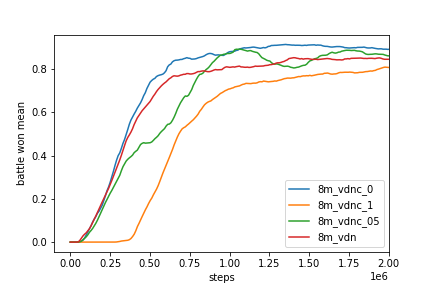
\includegraphics[width=\textwidth]{img/results/vdnc_8m/battle_won_mean.png}
		\caption{Battle won mean}
	\end{subfigure}
	\hfill
	\begin{subfigure}[b]{0.49\textwidth}
		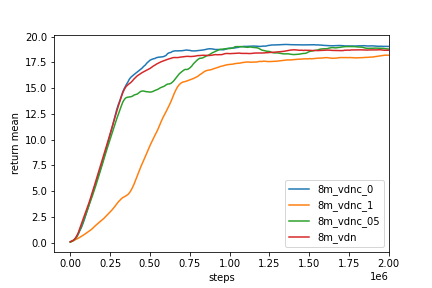
\includegraphics[width=\textwidth]{img/results/vdnc_8m/return_mean.png}
		\caption{Return mean}
	\end{subfigure}
	
	\caption{VDN on 8 marines vanilla vs. combined rewards c=0.0,0.5,1.0.}
	\label{fig:vdn_8m_results}
\end{figure}

As expected, environments with a larger group of agents profit from local rewards and gain even more from combined rewards. Vanilla VDN and combined reward VDN with $c=0$ are not able to win any rounds. Providing the agents with local rewards only ($c=1$) allows for at least some wins. 
%TODO: why just max 4% wins
%TODO: why fluctuating win rate
%TODO: why so late?
%TODO: why return c=0 != return vanilla
\begin{figure}[h!]
	  \centering
	\begin{subfigure}[b]{0.49\textwidth}
		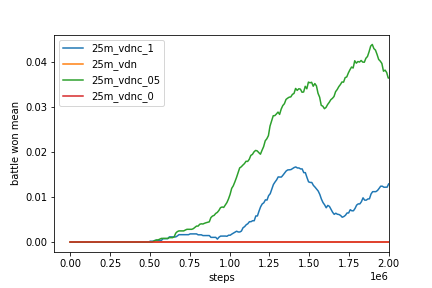
\includegraphics[width=\textwidth]{img/results/vdnc_25m/battle_won_mean.png}
		\caption{Battle won mean}
	\end{subfigure}
	\hfill
	\begin{subfigure}[b]{0.49\textwidth}
		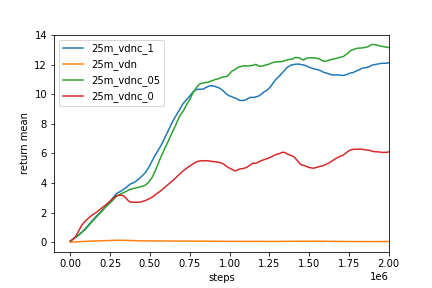
\includegraphics[width=\textwidth]{img/results/vdnc_25m/return_mean.png}
		\caption{Return mean}
	\end{subfigure}

	\caption{VDN on 25 marines vanilla vs. combined rewards c=0.0,0.5,1.0.}
	\label{fig:vdn_25m_results}
\end{figure}


All models and experiment metrics can be found at \url{https://github.com/PMatthaei/pymarl-results}. Further experiment permutations than the ones included in this documentation can be evaluated via the \href{https://github.com/PMatthaei/pymarl-results/blob/master/visualize_pymarl.ipynb}{visualization script in Google Colaboratory}.


\chapter{Conclusion}
 Problem: Environment $\rightarrow$ only homogeneous agents and symmetric groups. heterogeneous groups require more selfless behaviour f.e. tanking, exploding, being the bait.
 
\chapter{Future work}
The current implementation only used uniform unchangeable combine weights. Depending on the situation a agent might want to vary its combination to encourage a more selfish or more selfless behaviour.

Furthermore each agent should hold its own combination weight since their state may differ from other agents and requires a corresponding reward combination.

The current local reward function does not support heterogeneous team compositions since it is assumed every unit inflicts the same damage per step. This renders our implementation useless for a majority of environments.

Hyperparameter tuning not conducted.

\appendix
\chapter{Appendix}
\newpage
\section{SMAC - global reward function}
\label{sec:reward_global_python_code}
	\begin{python}
def global_reward(self):
	if self.reward_sparse:
		return 0
	
	reward, delta_deaths, delta_ally, delta_enemy = 0
	
	neg_scale = self.reward_negative_scale
	# update deaths
	for al_id, al_unit in self.agents.items():
		if not self.death_tracker_ally[al_id]:
		# did not die so far
		prev_health = (self.previous_ally_units[al_id].health			+ self.previous_ally_units[al_id].shield)
	if al_unit.health == 0:
		# just died
		self.death_tracker_ally[al_id] = 1
		if not self.reward_only_positive:
			delta_deaths -= self.reward_death_value * neg_scale
			delta_ally += prev_health * neg_scale
		else:
		# still alive
			delta_ally += neg_scale * (prev_health - al_unit.health - al_unit.shield)
	
	for e_id, e_unit in self.enemies.items():
		if not self.death_tracker_enemy[e_id]:
			prev_health = (
			self.previous_enemy_units[e_id].health
			+ self.previous_enemy_units[e_id].shield
			)
		if e_unit.health == 0:
			self.death_tracker_enemy[e_id] = 1
			delta_deaths += self.reward_death_value
			delta_enemy += prev_health
		else:
			delta_enemy += prev_health - e_unit.health - e_unit.shield
	# shield regeneration
	if self.reward_only_positive:
		reward = abs(delta_enemy + delta_deaths)  
	else:
		reward = delta_enemy + delta_deaths - delta_ally

return reward
	\end{python}
\newpage
\section{SMAC with combined rewards - local reward function} \label{sec:reward_local_python_code}
	\begin{python}
def local_reward(self, a_id, target_id):

	if self.reward_sparse:
		return 0

	neg_scale = self.reward_negative_scale
	delta_death, delta_self, delta_enemy = 0	
	agent_unit = self.get_unit_by_id(a_id)	
	# If the unit with id a_id is still alive
	if not self.death_tracker_ally[a_id]:
		# Fetch its previous health
		prev_health = self.previous_ally_units[a_id].health + self.previous_ally_units[a_id].shield
		# If it just died
		if agent_unit.health == 0:
		# Reward death negatively if configured
		if not self.reward_only_positive:
			delta_death -= self.reward_death_value * neg_scale
		# Remember lost health (= damage from enemies) to reward negatively later
			delta_self += prev_health * neg_scale
	# If still alive
	else:
		current_health = agent_unit.health + agent_unit.shield
		health_reward = prev_health - current_health
		# Reward the delta health (shield regeneration, heal through MMM)
		delta_self += neg_scale * health_reward
	
	# Search for the target (if it exists) which a_id attacked
	if target_id is not None:
		e_id, e_unit = next((e_id, _) for e_id, _ in self.enemies.items() if target_id == e_id)
		if not self.death_tracker_enemy[e_id]:
			# Reward dealt attack damage + kill
			delta_enemy += self.local_attack_r_t
	
	if self.reward_only_positive:
		reward = abs(delta_enemy + delta_death)
	else:
		reward = delta_enemy + delta_death - delta_self
	
	return reward
	\end{python}
\newpage
\section{Generalized reward combination function} \label{sec:reward_combination_code}
	\begin{python}
def combine_local_rewards(self, rs):
	ws = self.local_reward_weights
	# Pair local rewards with their weight
	rs_ws = list(zip(rs, ws))
	# Calculate weighted global reward
	r_global_combined = np.mean([(1.0 - w_j) * r_j for r_j, w_j in rs_ws])
	# Calculate each agents recombined reward
	rs_combined = [w_i * r_i + r_global_combined for r_i, w_i in rs_ws]
	
	return rs_combined
	\end{python}
